\chapter{路易斯结构与分子的形状}\label{ch:g10:lewis-and-shape}

二氧化碳分子呈直线形；水分子呈 V 形。
这一形状上的差异，是造成以下现象的原因之一：
水分子比二氧化碳分子轻，但水在室温下是液体，
二氧化碳却是气体。分子中的原子由共用电子结合在一起，
共用电子的方式
决定了分子的形状。本章画出共用电子，
并由此预测分子的形状。

\begin{recall}
价电子是最外层的电子；原子倾向于达到稀有气体的
构型，即最外层有八个电子（八隅规则），
氢则为两个电子（二隅规则）
（\cref{ch:g10:electron-shells}）。分子模型用小球表示原子，
用小棍表示化学键（\cref{ch:g7:atoms-and-molecules}）。
\end{recall}

\section{共价键}

\begin{definition}[共价键]\label{def:g10:lewis-and-shape:covalent-bond}
\emph{共价键}\index{共价键}是由两个原子共用的一对电子，
通常每个原子各提供该电子对中的一个电子。两个原子都把这一
共用电子对计入自身最外层，从而使二者达到
二隅或八隅结构。
\end{definition}

\begin{definition}[成键电子对与孤电子对]\label{def:g10:lewis-and-shape:lone-pair}
在分子中，每个原子的价电子都成对出现。
\emph{成键电子对}\index{成键电子对}为两个原子共用的电子对，并
形成共价键；\emph{孤电子对}\index{孤电子对}只属于单个原子，
不参与成键。
\end{definition}

\begin{proposition}[一个原子能形成几个共价键]\label{prop:g10:lewis-and-shape:valence}
原子形成的共价键数，与其为达到二隅或八隅结构
所缺少的电子数相同：
\begin{center}
\small
\begin{tabular}{lcccc}
\hline
原子 & 价电子数 & 键数 & 孤电子对数 & 示例 \\
\hline
H & 1 & 1 & 0 & \ce{H2} \\
C & 4 & 4 & 0 & \ce{CH4} \\
N & 5 & 3 & 1 & \ce{NH3} \\
O & 6 & 2 & 2 & \ce{H2O} \\
Cl & 7 & 1 & 3 & \ce{HCl} \\
\hline
\end{tabular}
\end{center}
\end{proposition}

\section{路易斯结构}

\begin{definition}[路易斯结构]\label{def:g10:lewis-and-shape:lewis-structure}
分子的\emph{路易斯结构}\index{路易斯结构}以元素符号表示其中的原子，
用两原子之间的一条线表示每个成键电子对，
用原子旁的一对小点表示每个孤电子对。
\end{definition}

\begin{definition}[双键与三键]\label{def:g10:lewis-and-shape:multiple-bond}
两个原子可以共用两对电子，即\emph{双键}\index{双键}，
以两条线表示；或共用三对电子，即\emph{三键}\index{三键}，
以三条线表示。
\end{definition}

\begin{method}[画路易斯结构]\label{met:g10:lewis-and-shape:draw}
\begin{enumerate}
  \item 将所有原子的价电子数相加，再取一半，得到
        电子对的数目。
  \item 用单键将原子相连（氢只形成一个键，
        总是位于外侧；碳通常位于中心）。
  \item 将剩余的电子对作为孤电子对放置，先放在外侧原子上，
        使其达到八隅结构。
  \item 若某原子仍缺少八隅结构，则将相邻原子的一个孤电子对
        变为第二个（或第三个）共用电子对。
  \item 检查：每个氢原子有 2 个电子，其他每个原子有 8 个电子，且
        所有电子对都已用完。
\end{enumerate}
\end{method}

\begin{example}[二氧化碳]\label{ex:g10:lewis-and-shape:co2}
\ce{CO2}：$4 + 2 \times 6 = 16$ 个价电子，共 8 对电子。单键
\ce{O-C-O} 使用 2 对电子；氧原子上的 6 对孤电子对使氧达到八隅结构，但
此时碳原子只有 4 个电子。若将每个氧原子的一个孤电子对
变为共用电子对，则得到两个双键：此时每个原子都达到八隅结构。
\end{example}

\begin{omfigure}
\setchemfig{atom sep=2.0em}
\begin{tabular}{cccccc}
\chemfig{H-H} & \chemfig{H-\charge{0=\:,90=\:,270=\:}{Cl}} & \chemfig{H-\charge{90=\:,270=\:}{O}-H} &
\chemfig{H-\charge{90=\:}{N}(-[6]H)-H} & \chemfig{H-C(-[2]H)(-[6]H)-H} &
\chemfig{\charge{135=\:,225=\:}{O}=C=\charge{45=\:,315=\:}{O}} \\[4pt]
\small \ce{H2} & \small \ce{HCl} & \small \ce{H2O} & \small \ce{NH3} & \small \ce{CH4} & \small \ce{CO2} \\[10pt]
\chemfig{\charge{180=\:}{N}~\charge{0=\:}{N}} & \chemfig{\charge{135=\:,225=\:}{O}=\charge{45=\:,315=\:}{O}} &
\chemfig{C(-[3]H)(-[5]H)=C(-[1]H)-[7]H} & \chemfig{H-C~\charge{0=\:}{N}} &
\chemfig{H-C(-[6]H)=\charge{45=\:,315=\:}{O}} & \\[4pt]
\small \ce{N2} & \small \ce{O2} & \small \ce{C2H4} & \small \ce{HCN} & \small 甲醛 \ce{CH2O} &
\end{tabular}

{\small 十一种分子的路易斯结构。除氢外，每个原子
周围都有四对电子（成键电子对与孤电子对），即八隅结构。}
\end{omfigure}

\section{分子的形状}

\begin{proposition}[电子对尽可能彼此远离]\label{prop:g10:lewis-and-shape:shape}
在中心原子周围，电子基团——即每个单键、双键或
三键，以及每个孤电子对——相互排斥，并尽可能远离地分布。
分子的形状由此决定：
\begin{center}
\small
\begin{tabular}{llll}
\hline
中心原子周围的电子基团数 & 其中孤电子对数 & 形状 & 示例 \\
\hline
2 & 0 & 直线形，键角 \ang{180} & \ce{CO2}、\ce{HCN} \\
3 & 0 & 平面三角形，键角 \ang{120} & \ce{CH2O}、\ce{C2H4} \\
4 & 0 & 四面体形，键角 \ang{109.5} & \ce{CH4} \\
4 & 1 & 三角锥形 & \ce{NH3} \\
4 & 2 & V 形 & \ce{H2O} \\
\hline
\end{tabular}
\end{center}
\end{proposition}
\admitted

\begin{remark}[这一规则的来源]\label{rem:g10:lewis-and-shape:vsepr}
这一规则只是一个模型，但对小分子的效果出奇地好；
它在本科一年级分册中得到了更精确的表述，并得到了部分解释。孤电子对
所占的空间比成键电子对略大，因此氨中的键角
（\ang{106.7}）和水中的键角（\ang{104.5}）都比甲烷的
\ang{109.5} 略小。
\end{remark}

\begin{omfigure}
\begin{tikzpicture}[font=\small]
  % methane, tetrahedral, in perspective
  \begin{scope}
    \node[aC] (c) at (0,0) {};
    \node[aH, minimum size=3.6mm] (hb) at (0.3,-0.12) {};
    \node[aH] (h1) at (0,1.05) {};
    \node[aH] (h2) at (-1.0,-0.45) {};
    \node[aH] (h3) at (0.72,-0.5) {};
    \begin{scope}[on background layer]
      \foreach \h in {h1,h2,h3,hb} \draw[bond] (c.center) -- (\h.center);
    \end{scope}
    \node[aC] at (0,0) {};
    \node at (0,-1.35) {甲烷：四面体形};
    \node[font=\footnotesize] at (-0.55,0.55) {\ang{109.5}};
  \end{scope}
  % ammonia, pyramid
  \begin{scope}[xshift=4.2cm]
    \fill[omDef!25] (0,0.2) ellipse (0.18 and 0.45);
    \node[font=\scriptsize, omDef] at (0,1.0) {孤电子对};
    \node[aN] (n) at (0,0) {};
    \node[aH] (h1) at (-0.95,-0.5) {};
    \node[aH] (h2) at (0.7,-0.55) {};
    \node[aH, minimum size=3.6mm] (h3) at (0.25,-0.2) {};
    \begin{scope}[on background layer]
      \foreach \h in {h1,h2,h3} \draw[bond] (n.center) -- (\h.center);
    \end{scope}
    \node[aN] at (0,0) {};
    \node at (0,-1.35) {氨：三角锥形};
  \end{scope}
  % water, bent
  \begin{scope}[xshift=8.4cm]
    \fill[omDef!25, rotate=25] (0,0.2) ellipse (0.16 and 0.42);
    \fill[omDef!25, rotate=-25] (0,0.2) ellipse (0.16 and 0.42);
    \node[aO] (o) at (0,0) {};
    \node[aH] (h1) at (-0.8,-0.58) {};
    \node[aH] (h2) at (0.8,-0.58) {};
    \begin{scope}[on background layer]
      \draw[bond] (o.center) -- (h1.center); \draw[bond] (o.center) -- (h2.center);
    \end{scope}
    \node[aO] at (0,0) {};
    \draw[black!60] (-0.32,-0.23) arc[start angle=216, end angle=324, radius=0.4];
    \node[font=\footnotesize] at (0,-0.65) {\ang{104.5}};
    \node at (0,-1.35) {水：V 形};
  \end{scope}
  % carbon dioxide, linear
  \begin{scope}[xshift=12.0cm]
    \node[aO] (a) at (-0.8,0) {}; \node[aC] (c) at (0,0) {}; \node[aO] (b) at (0.8,0) {};
    \begin{scope}[on background layer]
      \foreach \d in {-1.6,1.6} {
        \draw[bond, line width=1.1pt] ([yshift=\d pt]a.center) -- ([yshift=\d pt]c.center);
        \draw[bond, line width=1.1pt] ([yshift=\d pt]c.center) -- ([yshift=\d pt]b.center);}
    \end{scope}
    \node at (0,-1.35) {二氧化碳：直线形};
  \end{scope}
\end{tikzpicture}

{\small 四种分子的形状（阴影瓣表示孤电子对）。
% ledger: ang:H2O, ang:NH3
甲烷为四面体，氨为三角锥形，水为 V 形，二氧化碳
为直线形。}
\end{omfigure}

\begin{omfigure}
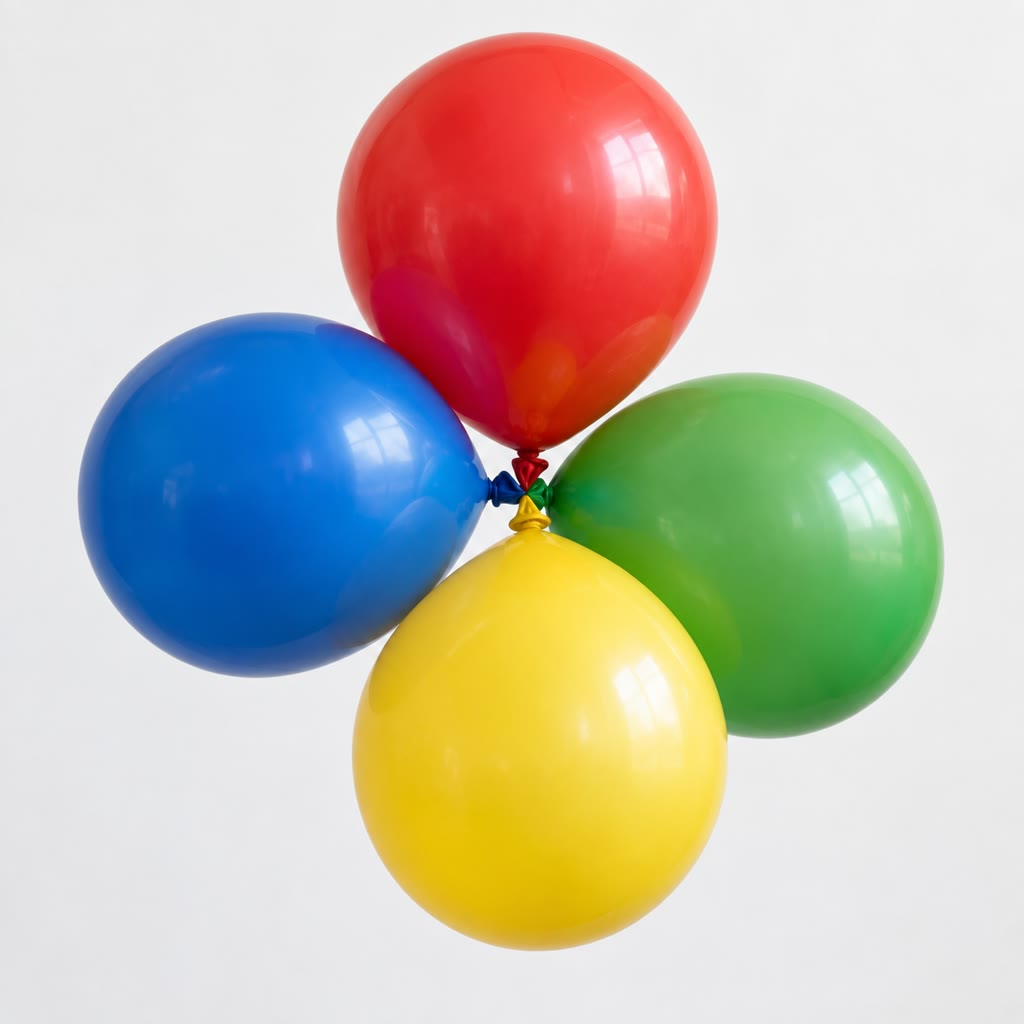
\includegraphics[width=0.38\linewidth]{images/book1/ai/g10-balloons-tetrahedron.jpg}

{\small 四个绑在一起的气球互相推挤，尽可能远离彼此；
在空间中它们指向四面体的顶点，
与碳原子周围的四个电子对类似。}
\end{omfigure}

\section{在空间中画分子}

\begin{notation}[楔形键与虚线键]\label{not:g10:lewis-and-shape:wedge}
要在平面纸上画出空间中的分子，位于纸面内的键
画成普通线条，指向读者的键画成实心楔形，
背离读者的键画成虚线楔形。甲烷的画法如下：
两个键位于纸面内，一个指向读者，一个背离读者。
\begin{center}
\chemfig{C(-[2]H)(-[4]H)(<[7]H)(<:[5]H)}
\end{center}
\end{notation}

\section{练习}

\begin{exercise}[$\star$]\label{exo:g10:lewis-and-shape:1}
什么是共价键？什么是孤电子对？
\end{exercise}

\begin{exercise}[$\star$]\label{exo:g10:lewis-and-shape:2}
氢、碳、氮和氧通常各能形成几个共价键？
请用八隅规则和二隅规则加以说明。
\end{exercise}

\begin{exercise}[$\star$]\label{exo:g10:lewis-and-shape:3}
画出氯化氢 \ce{HCl} 的路易斯结构，并数一数
氯原子周围的电子数。
\end{exercise}

\begin{exercise}[$\star$]\label{exo:g10:lewis-and-shape:4}
\ce{NH3} 分子一共有多少个价电子？
共有多少个电子对？
\end{exercise}

\begin{exercise}[$\star$]\label{exo:g10:lewis-and-shape:5}
给出 \ce{CH4}、\ce{NH3}、\ce{H2O} 和 \ce{CO2} 的形状。
\end{exercise}

\begin{exercise}[$\star\star$]\label{exo:g10:lewis-and-shape:6}
画出硫化氢 \ce{H2S} 的路易斯结构（硫与氧同族），
并预测其形状。
\end{exercise}

\begin{exercise}[$\star\star$]\label{exo:g10:lewis-and-shape:7}
画出氮气 \ce{N2} 的路易斯结构，
按照方法逐步进行。
\end{exercise}

\begin{exercise}[$\star\star$]\label{exo:g10:lewis-and-shape:8}
画出甲醇 \ce{CH3OH} 的路易斯结构，
并给出碳原子和氧原子周围的形状。
\end{exercise}

\begin{exercise}[$\star\star$]\label{exo:g10:lewis-and-shape:9}
为什么 \ce{CO2} 是直线形而 \ce{H2O} 是角形，
尽管两者的中心原子都与另外两个原子相连？
\end{exercise}

\begin{exercise}[$\star\star$]\label{exo:g10:lewis-and-shape:10}
画出乙烯 \ce{C2H4} 的路易斯结构，
并给出每个碳原子周围的形状。
\end{exercise}

\begin{exercise}[$\star\star$]\label{exo:g10:lewis-and-shape:11}
画出四氯化碳 \ce{CCl4} 的路易斯结构，
并预测其形状。
\end{exercise}

\begin{exercise}[$\star\star\star$]\label{exo:g10:lewis-and-shape:12}
分子式为 \ce{C2H6O} 的分子有两种，分别画出其路易斯结构
（一种含 O--H 键，另一种含 C--O--C 链）。
\end{exercise}

\begin{exercise}[$\star\star\star$]\label{exo:g10:lewis-and-shape:13}
利用孤电子对解释：为什么氨的键角（\ang{106.7}）
小于甲烷的键角（\ang{109.5}），而水分子的键角（\ang{104.5}）
还要更小。
\end{exercise}

\begin{exercise}[$\star\star\star$]\label{exo:g10:lewis-and-shape:14}
画出氰化氢 \ce{HCN} 和甲醛 \ce{CH2O} 的路易斯结构，
并给出它们的形状。
\end{exercise}

\begin{exercise}[$\star\star\star$]\label{exo:g10:lewis-and-shape:15}
臭氧 \ce{O3} 是由三个氧原子连成的链状分子。数一数它的价电子对数，
画出路易斯结构，使每个氧原子都满足八隅规则
（一个双键、一个单键）。预测该分子是直线形
还是角形。
\end{exercise}

\section{问题：立方体中的分子}

\begin{problem}[{周末问题——设计分子模型套件中的碳球，
孔应当以多大角度钻出？}]
\label{pb:g10:lewis-and-shape:1}
% ledger: ang:H2O, ang:NH3
某公司生产分子模型套件。黑色碳球上必须钻出四个孔，
以使甲烷、乙烷及其他含碳分子
能呈现正确的形状。工程师用了一个技巧：正四面体
可以放入立方体内，其四个顶点分别位于立方体的四个顶点上，
且任意两个顶点不在同一条棱上。

\medskip
\noindent\textbf{第一部分——路易斯结构。}
\begin{enumerate}
  \item 画出甲烷 \ce{CH4}、氨 \ce{NH3} 和
        水 \ce{H2O} 的路易斯结构。
  \item 各自中心原子周围有多少组电子？
  \item 其中有多少组是孤电子对？
  \item 为什么碳球需要四个孔，
        而表示水的氧球只需两个孔？
  \item 乙烷 \ce{C2H6} 的模型用到两个碳球。画出它的路易斯结构，
        两个碳球之间用几根棍相连，
        还需要几个氢球？
\end{enumerate}

\medskip
\noindent\textbf{第二部分——形状。}
\begin{enumerate}[resume]
  \item 给出这三种分子各自的形状。
  \item 测得氨中的键角为 \ang{106.7}，水中的键角为 \ang{104.5}，
        解释它们为什么都小于甲烷的键角。
  \item 若要让模型显示真实的键角，
        水的氧球为什么不能简单地用一个碳球、空出两个孔来代替？
  \item 二氧化碳中，碳原子形成两个双键。在模型中，
        这两个双键之间应当相隔多大角度？
\end{enumerate}

\medskip
\noindent\textbf{第三部分——立方体。}
取边长为 $a$ 的立方体。碳原子位于其中心；
四个氢原子位于立方体的四个顶点上，且任意两个不在同一条棱上。
\begin{enumerate}[resume]
  \item 证明：这些氢原子中任意两个都位于某个面的一条对角线的两端。
        利用毕达哥拉斯定理，
        用 $a$ 表示它们之间的距离。
  \item 整个立方体的对角线（从一个顶点到相对的顶点）
        长为 $a\sqrt{3}$。由此推出碳原子
        到氢原子的距离。
  \item 在模型中取 $a = \qty{1}{cm}$，
        以厘米为单位给出两个距离，保留两位小数。
  \item 为什么四个 C--H 距离相等？
\end{enumerate}

\medskip
\noindent\textbf{第四部分——角度。}
碳原子 C 与两个氢原子 H$_1$、H$_2$ 构成一个等腰三角形。
设 M 为 H$_1$H$_2$ 的中点。
\begin{enumerate}[resume]
  \item 解释为什么三角形 C\,M\,H$_1$ 在 M 处是直角。
  \item 在这个直角三角形中，计算角
        $\widehat{\text{M\,C\,H}_1}$（即键角 H--C--H 的一半）的正弦值。
  \item 由此推出半角，再求出键角 H--C--H，
        保留一位小数。
  \item 与本章表格中的角度作比较。
  \item 说明碳球上的孔
        应当以多大角度钻出。
\end{enumerate}
\end{problem}
